\begin{frame}[containsverbatim]
\frametitle{Titelseiten}

\begin{itemize}
\item Titelseiten erscheinen standardmäßig so, wie es das Standard-Template
      von \LaTeX-Beamer vorsieht.
  \begin{itemize}
  \item Hierdurch können eine Reihe von Informationen wie Titel, Untertitel,
        Autoren, Institution, Logos, \dots\ übersichtlich dargestellt werden.
  \end{itemize}

\bigskip

\item Die CI sieht auch vor, dass auch lediglich der Präsentationstitel und ein
      Bild als Titelseite angezeigt werden können.
  \begin{itemize}
  \item Mittels \lstinline[language={[LaTeX]TeX}]+\setbeamertemplate{title page}[tucpicture]+
        wird auf das Titelbild-Layout umgeschaltet.
  \item Der Präsentationstitel wird wie gewöhnlich per 
        \lstinline[language={[LaTeX]TeX}]+\title{}+ festgelgt.
  \item Das Bild muss per \lstinline[language={[LaTeX]TeX}]+\titlegraphic{}+
        angegeben werden.
  \item Das Bild sollte auf die Breite \lstinline[language={[LaTeX]TeX}]+\hsize+
        skaliert werden.
  \item Das Bild sollte ein Seitenverhältnis von 7:3 haben.
  \end{itemize}
\end{itemize}
\end{frame}


\begin{frame}[containsverbatim]
\frametitle{Titelseiten (Beispiel)}

\begin{itemize}
\item Die folgende Beispieltitselseite wird durch folgenden Code generiert:

\begingroup
\small
\begin{lstlisting}[style=numberedblock,language={[LaTeX]TeX}]
\begingroup
\title{Demo-Titel}
\titlegraphic{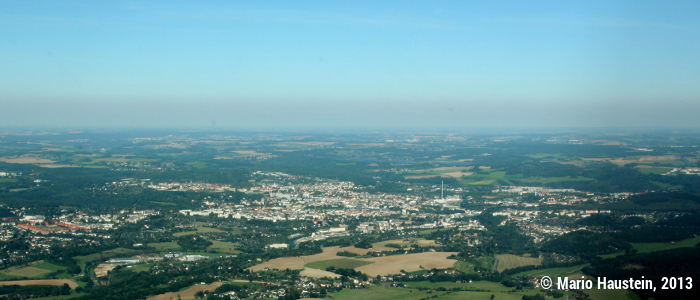
\includegraphics[width=\hsize]{bilder/titelbild}}

\setbeamertemplate{title page}[tucpicture]
\frame{\maketitle}
\endgroup
\end{lstlisting}
\endgroup

\bigskip

\item Anstatt \texttt{tucpicture} kann auch \texttt{tucnarrowpicture} angegeben werden.
  \begin{itemize}
  \item Das Titelbild erstreckt sich dann ggf. \structure{nicht} über die Logo-Spalte.
  \item Dies muss natürlich beim Seitverhältnis des Titelbilds berücksichtigt werden.
  \end{itemize}
\end{itemize}
\end{frame}


\tucthreeheadlines
\begingroup
\title{Demo-Titel}
\titlegraphic{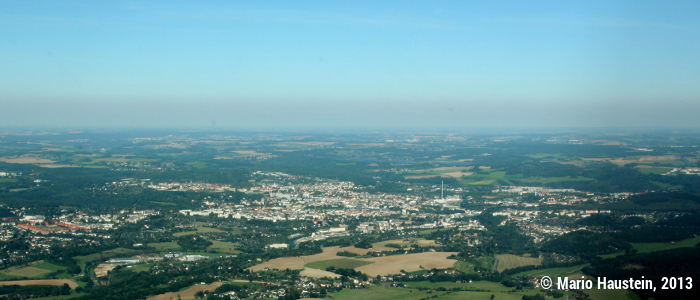
\includegraphics[width=\hsize]{bilder/titelbild}}

\setbeamertemplate{title page}[tucpicture]
\frame{\maketitle}
\endgroup
\tuctwoheadlines
